\documentclass[9pt]{article}
\usepackage[utf8]{inputenc}\usepackage[T1]{fontenc}\usepackage{lmodern}
\usepackage[letterpaper,top=.92cm,bottom=.92cm,left=1.05cm,right=1.05cm]{geometry}
\usepackage{graphicx,booktabs,amsmath,hyperref,array,tabularx,multicol,xcolor}
\definecolor{navy}{HTML}{102A43}\definecolor{blue}{HTML}{184E77}\definecolor{teal}{HTML}{2A9D8F}
\definecolor{pale}{HTML}{EDF5FB}\definecolor{mint}{HTML}{DDF4EF}\definecolor{sand}{HTML}{FFF4D6}
\definecolor{red}{HTML}{C95745}\definecolor{ink}{HTML}{172033}\definecolor{muted}{HTML}{526B7A}
\hypersetup{colorlinks=true,urlcolor=blue,linkcolor=blue,pageanchor=false}
\setlength{\parindent}{0pt}\setlength{\parskip}{2.4pt}\setlength{\tabcolsep}{3.5pt}\renewcommand{\arraystretch}{1.08}
\newcolumntype{Y}{>{\raggedright\arraybackslash}X}
\newcommand{\pagetitle}[2]{{\color{navy}\LARGE\bfseries #1\par}\vspace{1pt}{\color{teal}\rule{\linewidth}{1.5pt}}\vspace{1pt}{\color{muted}\small #2\par}\vspace{4pt}}
\newcommand{\takeaway}[1]{\par\noindent\textcolor{navy}{\textbf{Conclusión.} #1}\par}
\newcommand{\warn}[1]{\par\noindent\textcolor{red}{#1}\par}
\newcommand{\subhead}[1]{\vspace{2pt}{\color{blue}\bfseries #1}\par}
\begin{document}

% 1 — PORTADA
\begin{titlepage}\pagecolor{navy}\color{white}
\vspace*{.25cm}{\small\bfseries DEEP LEARNING Y SISTEMAS INTELIGENTES\hfill PROYECTO 1 · V6\par}
\vspace{.35cm}{\color{teal}\rule{\linewidth}{2pt}}\vspace{.7cm}
{\Huge\bfseries Monitoreo transaccional\par}\vspace{.15cm}{\LARGE Evidencia del valor del orden y detección de anomalías\par}
\vspace{.65cm}{\large\bfseries Pregunta ejecutiva\par}\vspace{3pt}¿El orden, una arquitectura secuencial o un encoder--decoder detectan fraude mejor que un baseline tabular competitivo?
\vspace{.65cm}\begin{tabularx}{\linewidth}{@{}XXXX@{}}
\centering\textbf{590,540}\newline\scriptsize transacciones&\centering\textbf{3.50\%}\newline\scriptsize fraude&\centering\textbf{0.559}\newline\scriptsize AP A histórico&\centering\textbf{0.807}\newline\scriptsize recall A histórico
\end{tabularx}
\vspace{.7cm}{\color{teal}\Large\bfseries Decisión: conservar A\par}\vspace{4pt}A mantiene el mejor soporte interno para la decisión. C no cumple su regla previa; B no demuestra valor del orden; D detecta anomalías con demasiadas falsas alarmas. El benchmark se reporta descriptivamente, no se usa para reescribir el veredicto.
\vfill\begin{tabularx}{\linewidth}{@{}YY@{}}\textbf{Universidad del Valle de Guatemala}\newline Facultad de Ingeniería · Sección 30\newline Docente: Kevin Recinos · Semestre II 2026&\textbf{Equipo}\newline Wilson Alejandro Calderón Argueta · 22018\newline Pablo Daniel Barillas Moreno · 22193\end{tabularx}
\end{titlepage}\hypersetup{pageanchor=true}\setcounter{page}{1}\nopagecolor\color{ink}

% 2 — DATOS
\pagetitle{1 · Integridad de datos, EDA y protocolo temporal}{La calidad del experimento depende más de causalidad, identidad y representación que del tamaño de la red.}
\takeaway{Se usaron todas las 590,540 transacciones. Los IDs son llaves, no predictores; las variables históricas excluyen el evento actual y las transformaciones se ajustan solo con train.}
\begin{multicols}{2}
\subhead{Fuente y población} Los datos proceden de \href{https://www.kaggle.com/competitions/ieee-fraud-detection/overview}{IEEE--CIS Fraud Detection} en Kaggle, con transacciones anonimizadas suministradas por Vesta Corporation. \texttt{TransactionID} une las tablas y \texttt{TransactionDT} define el reloj. Hay 20,663 fraudes y prevalencia 3.50\%.

\subhead{Diagnóstico exploratorio} El cuaderno EDA audita faltantes, constantes, asociación con fraude, Spearman, PCA, deriva y cobertura de identidad. Encontró alta redundancia en el bloque V, pero PCA no se promueve por varianza explicada: en V3 redujo desempeño y puede borrar señal minoritaria. Se conservan variables por validación predictiva y estabilidad.

\subhead{Identidad proxy} La entidad \texttt{card1+card2+card3+card5+addr1} permite construir historia, pero puede mezclar clientes o fragmentar uno. La cobertura alcanza 76.3\% con al menos 8 eventos, 66.2\% con 16 y 55.3\% con 32.

\subhead{Causalidad} Para una transacción $t$, toda estadística satisface $x_t^{hist}=f(\{x_j:t_j<t\})$. Se añadieron conteos y montos de 1/6/24/72 horas, cambios de dispositivo/dirección, monto relativo, faltantes y variables C/D/V/identidad. No se usa partición aleatoria.
\end{multicols}
\subhead{Bloques cronológicos dentro del desarrollo}
\begin{tabularx}{\linewidth}{@{}p{2.2cm}p{2cm}Y Y@{}}\toprule
\textbf{Bloque}&\textbf{Fracción}&\textbf{Uso}&\textbf{Control}\\\midrule
Train&70\% total&Preprocesamiento y modelos base&Nunca observa validación\\
Early&0--35\% val&Early stopping de B/D&Anterior a toda selección\\
Meta fit&35--50\% val&Controles/refuerzo A&No toca evaluación\\
Model select&50--60\% val&Selección A y B; ajuste C&A usa dos subventanas de estabilidad\\
Calibración&60--70\% val&Probabilidades&Separada del umbral\\
Umbral&70--80\% val&Costo con recall objetivo&Regla congelada\\
Evaluación&80--100\% val&Veredicto V6&No ajusta modelos\\
Benchmark&15\% total&Referencia histórica reutilizada&No es test ciego\\\bottomrule\end{tabularx}
\vfill\warn{\textbf{Integridad.} Imputación, escalado y vocabularios se aprenden con train. El benchmark ya fue observado en V1--V5; una confirmación exige una cohorte futura.}
\clearpage

% 3 — MODELOS Y RESULTADOS
\pagetitle{2 · Núcleo A/B, apuesta C y control D}{A/B/C usan las mismas filas, etiqueta, horizonte y puntajes continuos; D se añade como control de anomalía.}
\begin{tabularx}{\linewidth}{@{}p{.65cm}p{3.2cm}Y Y@{}}\toprule
&\textbf{Diseño}&\textbf{Qué prueba}&\textbf{Selección/entrenamiento}\\\midrule
A&LightGBM V4 y refuerzo causal&Capacidad sin leer orden&Se conserva \texttt{A\_V4}; el refuerzo no gana ambas subventanas\\
B&Embeddings + GRU o TCN causal&Dependencias de hasta 32 eventos&\texttt{B\_TCN} gana en model select\\
C&Logística sobre A/B/D y calidad&Complementariedad condicionada&Regla previa: $+0.01$ AP, $-5\%$ costo, recall $\ge.75$\\
D&Autoencoder de legítimas&Anomalía por error de reconstrucción&Solo \texttt{isFraud=0} de train\\\bottomrule\end{tabularx}
\vspace{4pt}\subhead{Resultado común en evaluación interna}
\begin{center}\scriptsize\begin{tabular}{lrrrrrrr}\toprule Modelo&AP&ROC&Prec.&Recall&F1&Costo&Alertas/100k\\\midrule
A&0.536&0.901&0.147&0.803&0.249&Q904,620&16,741\\
B&0.392&0.853&0.111&0.713&0.192&Q1,215,540&19,761\\
C&0.519&0.902&0.165&0.774&0.273&Q898,920&14,365\\
D&0.217&0.758&0.054&0.744&0.101&Q1,852,080&42,056\\
\bottomrule\end{tabular}\end{center}
\begin{minipage}[c]{.60\linewidth}\centering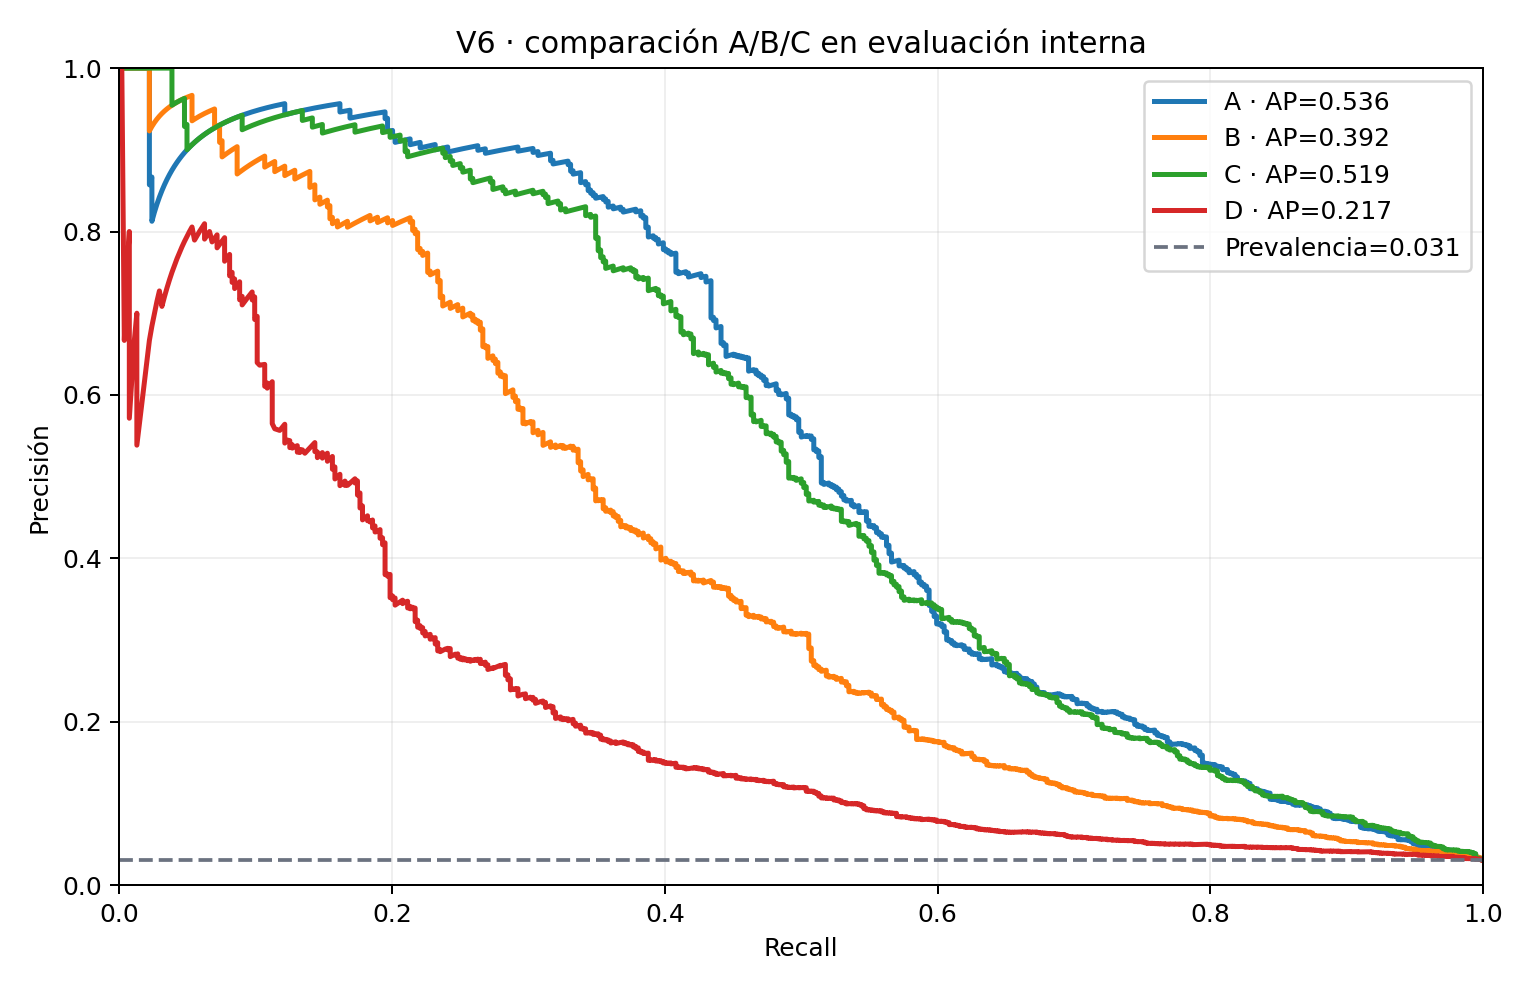
\includegraphics[width=\linewidth]{../../../evidencia/figuras/v6/01_comparacion_abc_validacion.png}\end{minipage}\hfill
\begin{minipage}[c]{.37\linewidth}\small
\textbf{AP} resume precisión al recorrer recall y es principal por el desbalance. \textbf{ROC--AUC} mide ordenamiento positivo--negativo, pero una tasa pequeña de FP aplicada a muchos legítimos todavía genera miles de alertas. \textbf{Precisión} es pureza de alertas; \textbf{recall} es cobertura de fraude; \textbf{F1} no incorpora quetzales.

A logra AP 0.536. C mejora precisión y F1 frente a A, pero pierde AP; D alcanza recall 0.744 a costa de precisión 0.054. Ese patrón confirma que detectar rareza no basta.
\end{minipage}
\vfill\takeaway{A conserva el ranking más defendible. C compra eficiencia de alertas, pero no alcanza el criterio congelado. D produce demasiadas falsas alarmas para ser candidato.}
\clearpage

% 4 — ORDEN
\pagetitle{3 · ¿El orden aporta?}{Una red secuencial no demuestra uso del orden por arquitectura; debe degradarse cuando el orden se destruye.}
\begin{minipage}[c]{.62\linewidth}\centering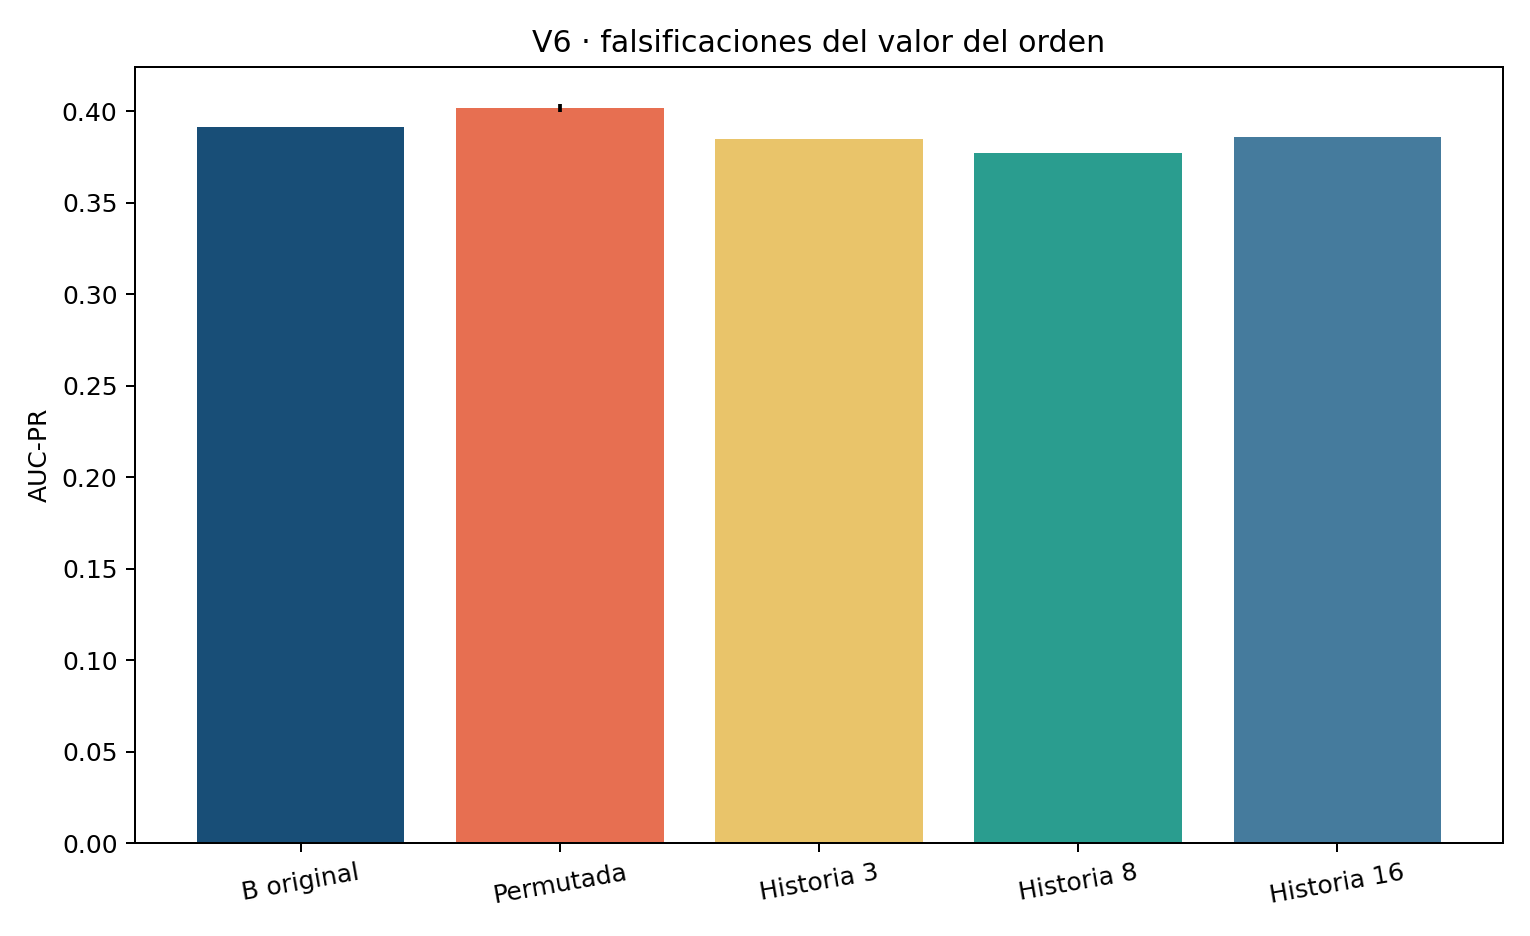
\includegraphics[width=\linewidth]{../../../evidencia/figuras/v6/03_falsificaciones_orden_v6.png}\end{minipage}\hfill
\begin{minipage}[c]{.35\linewidth}\small\begin{tabularx}{\linewidth}{@{}Y r@{}}\toprule Condición&AP\\\midrule
B original&0.3915\\ Permutada&0.4016$\pm$0.0023\\ Historia 3&0.3847\\ Historia 8&0.3774\\ Historia 16&0.3860\\\bottomrule\end{tabularx}\end{minipage}
\subhead{Falsificación 1 · permutación controlada} Se conserva la transacción objetivo al final y se barajan únicamente sus antecedentes, con cinco semillas. La diferencia original--permutada es -0.0101 AP. Como es negativa, destruir el orden mejora el ranking promedio; no se alcanza la caída material positiva predeclarada de 0.01.

\subhead{Falsificación 2 · longitud de historia} Recortar a 3, 8 o 16 eventos tampoco revela una ventaja creciente y estable. La ventana completa de 32 no domina claramente a las variantes cortas. Esto es coherente con una identidad proxy ruidosa: más eventos pueden añadir operaciones de otra persona o patrones legítimos no transferibles.

\subhead{Interpretación} B sí contiene información predictiva: AP 0.392 supera ampliamente la prevalencia. Lo que falla es la afirmación causal estrecha de que el \emph{orden} explica esa utilidad. B puede apoyarse en el evento actual, composición del historial y variables agregadas por evento.

\begin{tabularx}{\linewidth}{@{}p{3cm}Y Y@{}}\toprule Pregunta&Resultado&Conclusión permitida\\\midrule
¿B predice mejor que azar?&Sí, AP mayor que prevalencia&B aprende señal\\
¿B supera A?&No, pierde 0.145 AP&A sigue siendo más competitivo\\
¿B usa favorablemente el orden?&No; permutar aumenta AP&No atribuir valor material al orden\\
¿Más historia ayuda?&Sin patrón monotónico&No aumentar longitud sin mejor identidad\\\bottomrule\end{tabularx}
\vfill\takeaway{La prueba principal es negativa y concluyente dentro del alcance: con esta identidad, representación y arquitectura, el orden no aporta señal incremental demostrable.}
\clearpage

% 5 — D Y C
\pagetitle{4 · Encoder--decoder D y apuesta C}{El desbalance motiva modelar normalidad; la validación decide si la anomalía coincide con fraude.}
\begin{multicols}{2}
\subhead{Diseño de D} El encoder comprime las variables numéricas estandarizadas y el decoder reconstruye la transacción. Se entrena únicamente con legítimas de train y minimiza
\[\mathcal L_{AE}=\frac1p\sum_{j=1}^p(x_j-\hat x_j)^2.\]
El MSE final sobre legítimas tempranas es 0.0382. El error se transforma en percentil frente a 120 mil errores legítimos de referencia y luego se calibra.

\subhead{Qué obtuvo D} Internamente, D logra ROC 0.758 y recall 0.744, pero AP 0.217, precisión 0.054 y 42,056 alertas/100k. Muchos eventos legítimos raros parecen anomalías; faltantes y deriva también elevan reconstrucción.

\subhead{Apuesta C} C recibe logits A/B/D, calidad de historia, identidad disponible, monto, longitud, producto y faltantes. Se ajusta en model select, se calibra después y nunca observa evaluación al aprender pesos.

\subhead{Veredicto congelado} Frente a A, C cambia AP en -0.0170, reduce costo 0.63\% y alcanza recall 0.774. Requería $+0.01$ AP, $-5\%$ costo y recall $\ge.75$. Solo cumple recall: \textbf{C no es útil según su hipótesis}.
\end{multicols}
\begin{minipage}[c]{.48\linewidth}\centering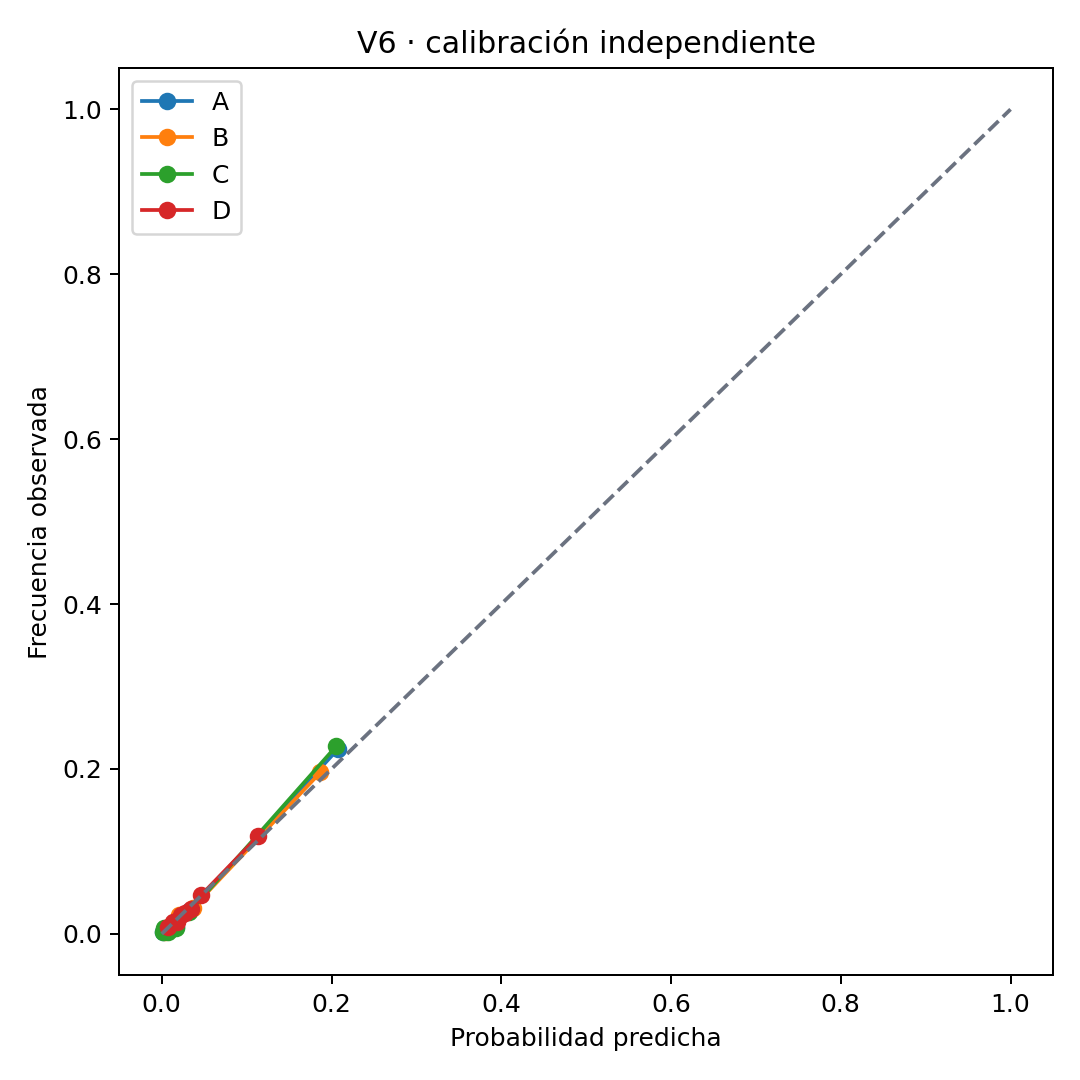
\includegraphics[width=.92\linewidth]{../../../evidencia/figuras/v6/05_calibracion_v6.png}\end{minipage}\hfill
\begin{minipage}[c]{.49\linewidth}\small
\textbf{Calibración.} Un score de ranking no es automáticamente una probabilidad. Cada modelo usa calibración logística en un bloque separado. Se compara Brier antes/después; el umbral económico se fija en el bloque siguiente.

\textbf{Lectura responsable.} El autoencoder es una ablation informativa, no un fracaso inútil: demuestra que la clase legítima es multimodal y temporalmente cambiante. Para mejorarlo se requerirían autoencoders por segmento, pérdidas robustas, categorías embebidas y validación de deriva; no basta aumentar capas.
\end{minipage}
\vfill\warn{\textbf{No seleccionar con el benchmark.} Aunque C aparece descriptivamente competitivo en el período histórico final, la hipótesis se juzga en evaluación interna y permanece rechazada.}
\clearpage

% 6 — ECONOMÍA
\pagetitle{5 · Umbral, benchmark histórico y operación}{El costo hace explícito el intercambio: un falso negativo vale 23.3 veces un falso positivo.}
\[C(\tau)=Q4{,}200\,FN(\tau)+Q180\,FP(\tau).\]
\begin{minipage}[c]{.55\linewidth}\centering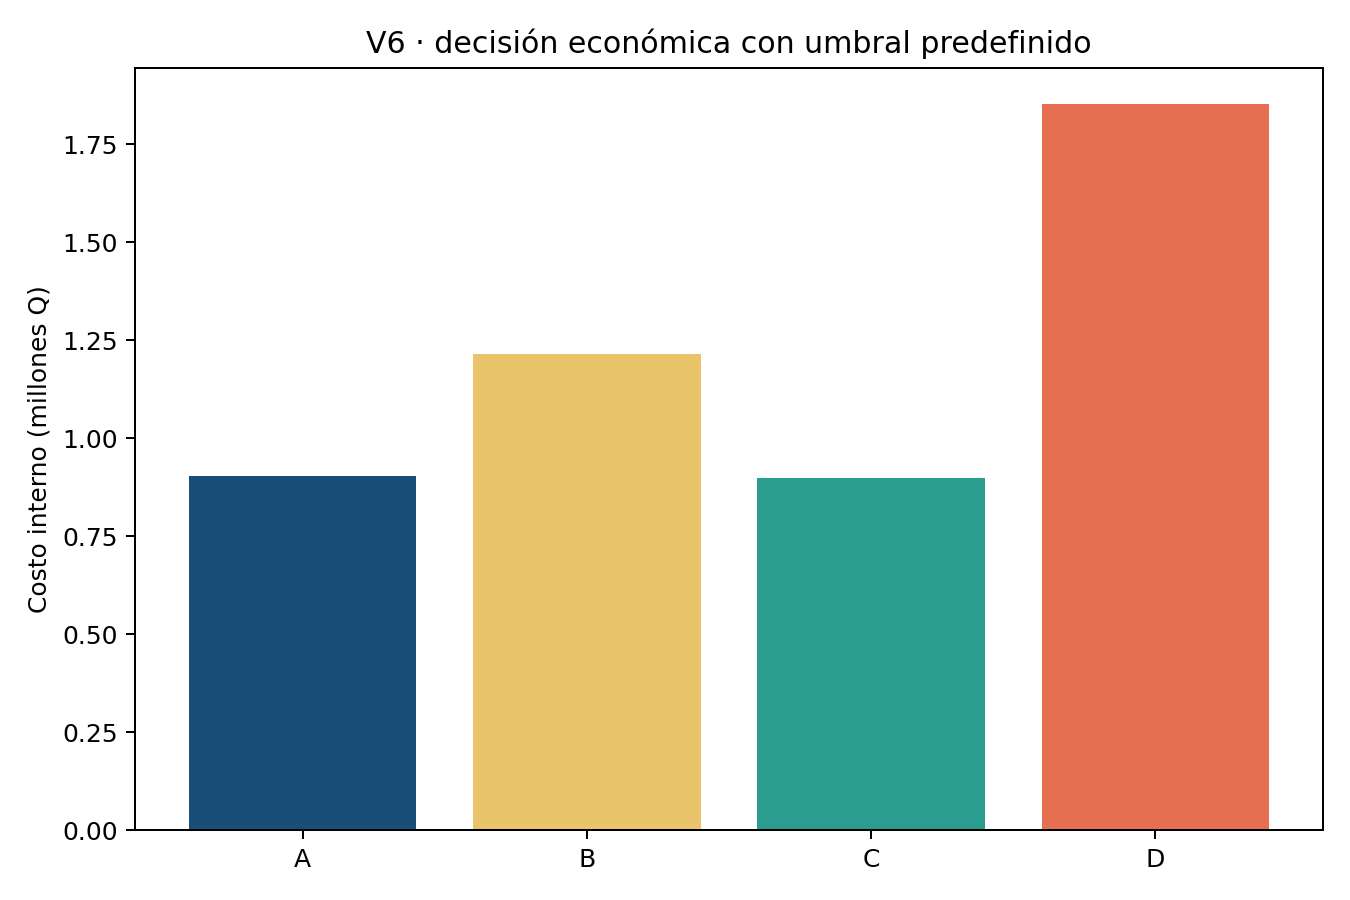
\includegraphics[width=\linewidth]{../../../evidencia/figuras/v6/04_costos_abc_v6.png}\end{minipage}\hfill
\begin{minipage}[c]{.42\linewidth}\small
A usa $\tau=0.03622$. En evaluación interna detecta 437 fraudes, omite 107 y produce 2529 falsas alarmas. Su costo es Q904,620, menor que B y D; C cuesta Q898,920, pero no cumple el criterio de ranking.

El recall alto de A (80.3\%) implica precisión moderada (14.7\%). No es contradicción: la política acepta falsas alarmas porque FN cuesta 23.3 veces FP.
\end{minipage}
\subhead{Benchmark temporal histórico reutilizado}
\begin{center}\scriptsize\begin{tabular}{lrrrrrrr}\toprule Modelo&AP&ROC&Prec.&Recall&F1&Costo&Alertas/100k\\\midrule
A&0.559&0.901&0.158&0.807&0.264&Q4,889,400&17,801\\
B&0.465&0.877&0.123&0.785&0.212&Q5,898,960&22,264\\
C&0.563&0.907&0.171&0.798&0.282&Q4,753,500&16,207\\
D&0.229&0.769&0.056&0.824&0.105&Q9,977,040&51,137\\
\bottomrule\end{tabular}\end{center}
\subhead{Qué significan las cifras} A alcanza AP 0.559 y ROC 0.901: ordena razonablemente el riesgo, pero solo 15.8\% de sus alertas es fraude. Detecta 80.7\% de fraudes y genera 17,801 alertas por 100 mil. C luce mejor en AP histórico, pero esa observación es exploratoria; promoverlo ahora reutilizaría el benchmark.

\subhead{Errores y sensibilidad} Los falsos negativos de mayor monto se guardan para revisión. La proyección mensual usa 1.4 millones de tarjetas y escenarios 5/12/20 transacciones por tarjeta; no es una cifra contable. Cambios en costo FN/FP o capacidad de analistas pueden mover el umbral sin modificar AP.
\vfill\takeaway{Las métricas son defendibles, no perfectas: A prioriza fraude mejor que azar y cubre cerca de 81\%, pero la baja precisión confirma una carga relevante de falsas alarmas.}
\clearpage

% 7 — CIERRE
\pagetitle{6 · Matriz de evidencias, decisión y límites}{Cada afirmación se vincula con una prueba y declara qué evidencia podría cambiarla.}
\scriptsize\begin{tabularx}{\linewidth}{@{}p{2.2cm}p{2.6cm}Y Y@{}}\toprule Evidencia&Artefacto&Conclusión&Limitación\\\midrule
Integridad&EDA, particiones, contrato&590,540 filas; causalidad y train-only&Identidad aproximada\\
A/B común&Figura 1 y scores&A supera B en AP y costo&Ingeniería de A más rica\\
Valor del orden&5 permutaciones; 3/8/16&Permutar no perjudica; sin evidencia de orden&Una proxy y dos arquitecturas\\
Apuesta C&JSON de hipótesis&No alcanza +0.01 AP ni 5\% ahorro&Fusión logística específica\\
Encoder--decoder&Checkpoint y score D&Anomalía tiene recall, no precisión&Normalidad multimodal y deriva\\
Economía&Curvas y Figura 4&A minimiza costo entre candidatos válidos&Costos/volumen académicos\\
Recomendación&Contrato/manifiesto&Conservar A como candidato V6&Confirmar en cohorte futura\\\bottomrule\end{tabularx}
\subhead{Decisión concluyente} Conservar A. No promover B porque no supera A ni demuestra valor del orden. No promover C porque incumple la hipótesis previa, aunque el benchmark motive investigarlo en una cohorte nueva. No promover D porque su precisión y costo son inaceptables. La siguiente iteración debe priorizar identidad bancaria fiable, variables categóricas completas, validación walk-forward y una nueva cohorte etiquetada.

\subhead{Qué cambiaría la decisión} (1) caída AP $\ge0.01$ al permutar con una identidad fiable; (2) C cumpliendo simultáneamente ganancia AP, ahorro y recall en ventanas walk-forward; (3) D reduciendo alertas sin perder cobertura; (4) costos operativos reales que cambien el umbral; (5) estabilidad en una cohorte futura congelada.

\subhead{Límites} Datos anonimizados; identidad proxy; benchmark reutilizado; costo académico; sin auditoría productiva de privacidad, equidad, explicabilidad, deriva, seguridad adversarial ni latencia. Los scores indican riesgo estadístico, no certeza de fraude.

\subhead{Uso de inteligencia artificial} Se utilizó asistencia de IA para estructurar código, revisar consistencia, diseñar visuales y redactar documentación. Los autores ejecutaron el pipeline, verificaron IDs, particiones, métricas, falsificaciones, artefactos y conclusiones, y deben poder defender las decisiones.

\subhead{Referencias APA 7} \scriptsize
IEEE Computational Intelligence Society. (2019). \textit{IEEE--CIS Fraud Detection} [Data set]. Kaggle. \url{https://www.kaggle.com/competitions/ieee-fraud-detection/overview}\\
Ke, G., et al. (2017). LightGBM: A highly efficient gradient boosting decision tree. \textit{Advances in Neural Information Processing Systems, 30}.\\
Saito, T., \& Rehmsmeier, M. (2015). The precision--recall plot is more informative than the ROC plot when evaluating binary classifiers on imbalanced datasets. \textit{PLOS ONE, 10}(3), e0118432. \url{https://doi.org/10.1371/journal.pone.0118432}\\
Zhou, C., \& Paffenroth, R. C. (2017). Anomaly detection with robust deep autoencoders. \textit{Proceedings of KDD}, 665--674. \url{https://doi.org/10.1145/3097983.3098052}
\vfill\takeaway{V6 mejora el rigor más que la cifra: prueba más modelos, rechaza mejoras inestables y conserva únicamente la decisión respaldada por evaluación temporal interna.}
\end{document}
